\documentclass[ignorenonframetext,notheorems,hidelinks,aspectratio=1610]{beamer}
%\usetheme[compress]{JuanLesPins}
\usetheme{JuanLesPins}
\usecolortheme{iwr}
\usepackage{mathsim}
\lstset{language=Python}
\usetikzlibrary{snakes}
\usetikzlibrary{matrix,fit}
\pgfdeclarelayer{bg}
\pgfsetlayers{bg,main}
\tikzset{velox/.style={color=black,draw,fill=red,thick,%
    shape=diamond,aspect=.4,
    inner sep=1.3pt,transform shape}}
\tikzset{veloy/.style={color=black,draw,fill=red,thick,%
    shape=diamond,aspect=2.5,
    inner sep=1.3pt,transform shape}}
\tikzset{veloxy/.style={color=black,draw,fill=red,thick,%
    shape=star,star points=4,star point ratio=2.2,
    inner sep=1.3pt,transform shape}}
\tikzset{pressure/.style={color=black,draw,fill=cyan,thick,%
    shape=circle,inner sep=2pt,transform shape}}
\tikzset{velo/.style={transform shape,double=red,arrows={-Stealth[open,fill=red]}}}

%% Macros for drawing degrees of freedom for different shapes/elements.
%% Arguments are always:
%%   #1: Starting point
%%   #2: End point
%%   #3: polynomial degree
%%   #4: node settings

\tikzset{pics/edgenormal/.style args={#1/#2/#3/#4}{%
    code={%
      \draw #1 -- #2
      node foreach \x [evaluate=\x as \xval] in {1,...,#3} [#4,sloped,pos=\xval/(#3+1)] {};
      }
}}


%% Macros for drawing degrees of freedom for different shapes/elements.
%% Arguments are always:
%%   #1: polynomial degree
%%   #2: node settings

\tikzset{pics/tripile/.style args={#1/#2}{%
    code={%
      \coordinate (top) at (0,#1);
      \foreach \i in{0,...,#1}
      \foreach \j in{0,...,\i}
      {
        \tikzmath{
          \y = .3*(2/3*#1-\i)*cos(30);
          \x = .3*(\i/2-\j);
        }
        \node[#2] at (\x,\y) {};
      }
    }
}}

\tikzset{pics/tensor/.style args={#1/#2/#3}{%
    code={%
      \coordinate (top) at (0,#1);
      \foreach \i in{0,...,#1}
      \foreach \j in{0,...,#2}
      {
        \tikzmath{
          \y = 2*(\i+1)/(#1+2);
          \x = 2*(\j+1)/(#2+2);
        }
        \node[#3] at (\x,\y) {};
      }
    }
}}

\tikzset{pics/pfem/.style args={#1/#2}{%
    code={%
      \tikzmath{ \ytop=2*cos(30); }
      \coordinate (top) at (0,\ytop);

      \foreach \i in{0,...,#1}
      \foreach \j in{0,...,\i}
      {
        \tikzmath{
          \y = \ytop-\ytop*\i/#1;
          \x = 2*(\i/2-\j)/#1+1;
        }
        \node[#2] at (\x,\y) {};
      }
    }
}}

\tikzset{pics/qfem/.style args={#1/#2}{%
    code={%
      \foreach \i in{0,...,#1}
      \foreach \j in{0,...,#1}
      {
        \tikzmath{
          \y = 2-2*\i/#1;
          \x = 2-2*\j/#1;
        }
        \node[#2] at (\x,\y) {};
      }
    }
}}

%%% Local Variables:
%%% mode: latex
%%% TeX-master: "all"
%%% End:

\def\esp#1{V_{#1}}

\usepackage{times}
\usepackage{xr}
\externaldocument{main}
\usepackage{mfirstuc}
\usepackage{mathtools}  
\mathtoolsset{showonlyrefs}

\newcommand{\rd}{\operatorname{rd}}

\def\footnote#1{}
\def\putindex#1{#1}
\title{Numerical Linear Algebra}
\author{Guido Kanschat}
\date{\today}
\begin{document}
\frame{\maketitle}
\frame{\frametitle{Overview}\tableofcontents[hideallsubsections]}
\section{Dense Algebraic Eigenvalue Problems}
\frame{\sectoc}

\subsection{Mathematical background}
\subsubsection{Definition of EVP}
\frame{\subsubtoc}
\frame {\input {blocks/Definition-eigenvalue.tex}}
\frame {\input {blocks/Definition-eigenvalue-algebraic.tex}
  \pause
  \input {blocks/Lemma-eigenvalue-equivalent.tex}}
\frame {\input {blocks/Theorem-eigenvalue-count.tex}
  \pause
  \input {blocks/Definition-eigenvalue-simple.tex}}
\frame {\input {blocks/Definition-right-left-ev.tex}
\input {blocks/Lemma-eigenvalues-conjugate.tex}}

\subsubsection{Bases and matrices}
\frame{\subsubtoc}
\frame {\input {blocks/Notation-column-vectors.tex}}
\frame {\input {blocks/Notation-matrix-linear-combination.tex}}
\frame {\input {blocks/Lemma-change-of-basis.tex}}
\frame {\input {blocks/Corollary-change-of-basis.tex}}
\frame {\input {blocks/Definition-similar-matrix.tex}
  \input {blocks/Lemma-similarity-equivalence.tex}}
\frame {\input {blocks/Lemma-matrix-basis-change.tex}}
\frame {\input {blocks/Theorem-Jordan-canonical-form.tex}}
\frame {\input {blocks/Definition-diagonalizable.tex}
  \input {blocks/Theorem-matrix-functions.tex}}
\frame {\input {blocks/Theorem-simultaneous-diagonalization.tex}}

\subsubsection{Normal and Hermitian matrices}
\frame{\subsubtoc}

\frame {\input {blocks/Definition-sesqui.tex}}
\frame {\input {blocks/Definition-inner-product.tex}
  \input {blocks/Example-Euclidean-ip.tex}}
\frame {\input {blocks/Definition-conjugate-matrix.tex}}
\frame {\input {blocks/Definition-orthonormal-unitary.tex}}

\frame {\input {blocks/Definition-normal-Hermitian.tex}}
\frame {\input {blocks/Lemma-Hermitian-eigenvalues-real.tex}
\input {blocks/Theorem-Hermitian-diagonalizable.tex}
\input {blocks/Corollary-symmetric-diagonalizable.tex}}
\frame {\input {blocks/Theorem-normal-diagonalizable.tex}}

\subsection{Well-posedness and bounds}
\frame{\subtoc}
\subsubsection{Bounds on eigenvalues}
\frame {\input {blocks/Definition-matrix-norm.tex}}
\frame {\input {blocks/Lemma-bound-by-norm.tex}}
\frame {\input {blocks/Lemma-pre-gershgorin.tex}}
\frame {\input {blocks/Theorem-gershgorin.tex}}
\subsubsection{The Rayleigh quotient}
\frame {\input {blocks/Definition-rayleigh-quotient.tex}}
\frame {\input {blocks/Theorem-minmax.tex}}

\subsubsection{Conditioning of the EVP}

\frame {\input {blocks/Definition-conditioning-eigenvalue.tex}}
\frame {\input {blocks/Example-characteristic-polynomial.tex}}
\frame {\input {blocks/Example-conditioning-Jordan-block.tex}
  \input {blocks/Theorem-Jordan-block-ill-conditioned.tex}}
\frame {\input {blocks/Theorem-bauer-fike.tex}
  \only<1>{\input {blocks/Definition-matrix-condition.tex}}
  \only<2>{\input {blocks/Corollary-conditioning-eigenvalues-normal.tex}}}
\frame {\input {blocks/Theorem-conditioning-eigenvalue-single.tex}}

\frame {\input {blocks/Example-conditioning-eigenvectors.tex}
  \pause
  \input {blocks/Remark-conditioning-eigenvectors.tex}}

\subsection{Vector iterations}
\frame{\subtoc}
\frame {\input {blocks/Algorithm-vector-iteration.tex}}
\frame {\input {blocks/Theorem-vector-iteration.tex}}
\frame {\input {blocks/Remark-vector-iteration.tex}}
\frame {\input {blocks/Lemma-Rayleigh-approximation.tex}}
\frame {\input {blocks/Algorithm-shifted-vector-iteration.tex}}
\frame {\input {blocks/Algorithm-inverse-iteration.tex}}
\frame {\input {blocks/Algorithm-Rayleigh-iteration.tex}}

\subsection{Subspace iterations, the QR-iteration}
\frame{\subtoc}

\subsubsection{Definition of the methods}
\frame {\input {blocks/Algorithm-subspace-iteration.tex}}
\frame {\input {blocks/Algorithm-gram-schmidt.tex}
  \input {blocks/Theorem-gram-schmidt.tex}}

\frame {\input {blocks/Definition-qr-decomposition.tex}}
\frame {\input {blocks/Lemma-qr-columns.tex}
  \input {blocks/Theorem-qr-existence.tex}}
\frame {\input {blocks/Algorithm-qr-iteration.tex}}

\frame {\input {blocks/Theorem-schur-canonical.tex}}
\frame {\input {blocks/Lemma-schur-canonical-1.tex}}
\frame {\input {blocks/Lemma-schur-canonical-2.tex}}

\frame {\input {blocks/Definition-dominant-invariant-subspace.tex}}
\frame {\input {blocks/Definition-projection-distance.tex}
  \input {blocks/Example-projection-distance.tex}}

\frame {\input {blocks/Theorem-convergence-subspace-iteration.tex}}

\frame {\input {blocks/Algorithm-qr-iteration.tex}
  \input {blocks/Lemma-qr-1.tex}}

\subsubsection{Implementation issues}
\frame{\subsubtoc}
\frame {\input {blocks/Definition-householder-transformation.tex}}
\frame {\input {blocks/Lemma-householder-symmetry.tex}}
\frame {\input {blocks/Lemma-householder-qr.tex}}
\frame {\input {blocks/Algorithm-householder-multiplication.tex}}

\frame {\input {blocks/Definition-givens.tex}}
\frame {\input {blocks/Lemma-givens-computation.tex}}
\frame {\input {blocks/Definition-givens-complex.tex}}
\frame {\input {blocks/Lemma-givens-computation-complex.tex}}
\frame {\input {blocks/Algorithm-givens-multiplication.tex}}

\frame {\input {blocks/Definition-hessenberg.tex}}
\frame {\input {blocks/Algorithm-Hessenberg-qr.tex}}

\begin{frame}
  \frametitle{Example: 4-by-4-matrix}
  \begin{gather*}
    \matH \to \givens_{12}^*\matH
    \visible<2->{\to \givens_{23}^*\givens_{12}^*\matH}
    \visible<3->{\to \givens_{34}^*\givens_{23}^*\givens_{12}^*\matH = \matr}\\
    \visible<3->{\matr\matq = \matr\givens_{12}\givens_{23}\givens_{34}}\\
  \end{gather*}
    \only<1>{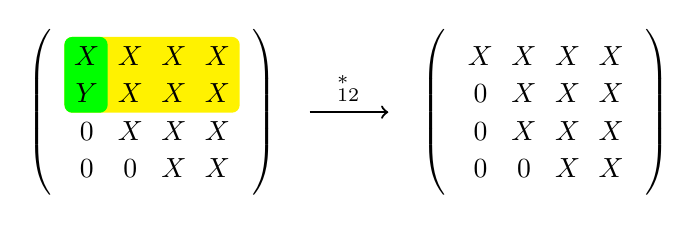
\begin{tikzpicture}\node
[matrix of math nodes,left delimiter=(,right delimiter=)] (m)  at (0,0)
{
  X&X&X&X\\
  Y&X&X&X\\
  0&X&X&X\\
  0&0&X&X\\
};

\node
[matrix of math nodes,left delimiter=(,right delimiter=)] (r)  at (5,0)
{
  X&X&X&X\\
  0&X&X&X\\
  0&X&X&X\\
  0&0&X&X\\
};

\draw[->,thick] (2,0) -- node[above] {$\matg_{12}^*\matH$} (3,0);

\begin{pgfonlayer}{bg}
  \node[fit={(m-1-1.north west) (m-2-4.south east)},fill=yellow,inner sep=0,rounded corners=1mm]{};
  \node[fit={(m-1-1.north west) (m-2-1.south east)},fill=green,inner sep=0,rounded corners=1mm]{};
\end{pgfonlayer}

;\end{tikzpicture}}
    \only<2>{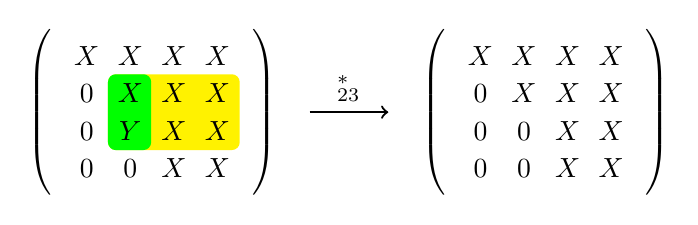
\begin{tikzpicture}\matrix
[matrix of math nodes,left delimiter=(,right delimiter=)] (m)
{
  X&X&X&X\\
  0&X&X&X\\
  0&Y&X&X\\
  0&0&X&X\\
};

\node
[matrix of math nodes,left delimiter=(,right delimiter=)] (r)  at (5,0)
{
  X&X&X&X\\
  0&X&X&X\\
  0&0&X&X\\
  0&0&X&X\\
};

\draw[->,thick] (2,0) -- node[above] {$\matg_{23}^*\matH$} (3,0);

\begin{pgfonlayer}{bg}
  \node[fit={(m-2-2.north west) (m-3-4.south east)},fill=yellow,inner sep=0,rounded corners=1mm]{};
  \node[fit={(m-2-2.north west) (m-3-2.south east)},fill=green,inner sep=0,rounded corners=1mm]{};
\end{pgfonlayer}
;\end{tikzpicture}}
    \only<3>{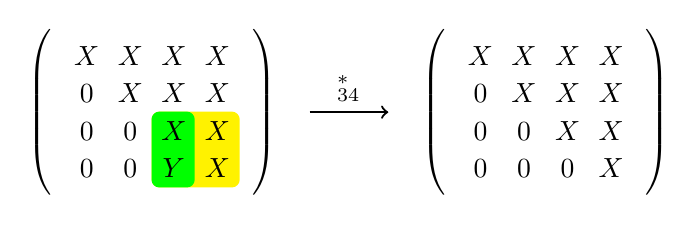
\begin{tikzpicture}\matrix
[matrix of math nodes,left delimiter=(,right delimiter=)] (m)
{
  X&X&X&X\\
  0&X&X&X\\
  0&0&X&X\\
  0&0&Y&X\\
};

\node
[matrix of math nodes,left delimiter=(,right delimiter=)] (r)  at (5,0)
{
  X&X&X&X\\
  0&X&X&X\\
  0&0&X&X\\
  0&0&0&X\\
};

\draw[->,thick] (2,0) -- node[above] {$\matg_{34}^*\matH$} (3,0);

\begin{pgfonlayer}{bg}
  \node[fit={(m-3-3.north west) (m-4-4.south east)},fill=yellow,inner sep=0,rounded corners=1mm]{};
  \node[fit={(m-3-3.north west) (m-4-3.south east)},fill=green,inner sep=0,rounded corners=1mm]{};
\end{pgfonlayer}
;\end{tikzpicture}}
    \only<4>{
      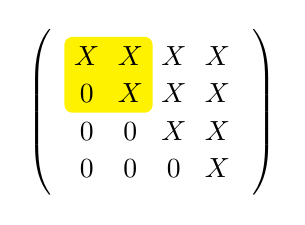
\begin{tikzpicture}\matrix
[matrix of math nodes,left delimiter=(,right delimiter=)] (m)
{
  X&X&X&X\\
  0&X&X&X\\
  0&0&X&X\\
  0&0&0&X\\
};
\begin{pgfonlayer}{bg}
  \node[fit={(m-1-1.north west) (m-2-2.south east)},fill=yellow,inner sep=0,rounded corners=1mm]{};
\end{pgfonlayer}
;\end{tikzpicture}
      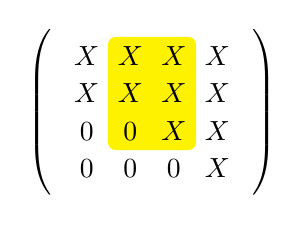
\begin{tikzpicture}\matrix
[matrix of math nodes,left delimiter=(,right delimiter=)] (m)
{
  X&X&X&X\\
  X&X&X&X\\
  0&0&X&X\\
  0&0&0&X\\
};
\begin{pgfonlayer}{bg}
  \node[fit={(m-1-2.north west) (m-3-3.south east)},fill=yellow,inner sep=0,rounded corners=1mm]{};
\end{pgfonlayer}
;\end{tikzpicture}
      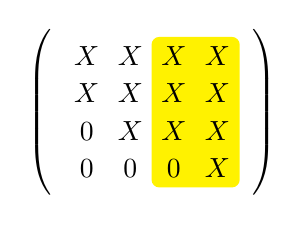
\begin{tikzpicture}\matrix
[matrix of math nodes,left delimiter=(,right delimiter=)] (m)
{
  X&X&X&X\\
  X&X&X&X\\
  0&X&X&X\\
  0&0&0&X\\
};
\begin{pgfonlayer}{bg}
  \node[fit={(m-1-3.north west) (m-4-4.south east)},fill=yellow,inner sep=0,rounded corners=1mm]{};
\end{pgfonlayer}
;\end{tikzpicture}
      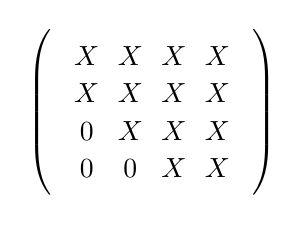
\begin{tikzpicture}\matrix
[matrix of math nodes,left delimiter=(,right delimiter=)] (m)
{
  X&X&X&X\\
  X&X&X&X\\
  0&X&X&X\\
  0&0&X&X\\
};
;\end{tikzpicture}}
  \end{frame}
\frame {\input {blocks/Theorem-Hessenberg-qr.tex}}
\frame {\input {blocks/Corollary-Hessenberg-qr.tex}}
\frame {\input {blocks/Theorem-Hessenberg-householder.tex}}

\frame {\input {blocks/Algorithm-qr-method.tex}}

\frame {\input {blocks/Theorem-hessenberg-qr-convergence.tex}}
\frame {\input {blocks/Theorem-qr-reduction.tex}
  \input {blocks/Definition-hessenberg-unreduced.tex}}

\subsubsection{Shitfs and deflation}

\frame {\input {blocks/Algorithm-shifted-qr-iteration.tex}
  \input {blocks/Lemma-shifted-qr-convergence.tex}}
\frame {\input {blocks/Example-rayleigh-shift.tex}}
\frame {\input {blocks/Definition-wilkinson-shift.tex}}
\frame {\input {blocks/Remark-wilkinson-shift.tex}}
\frame {\input {blocks/Algorithm-qr-deflation.tex}}
\frame {\input {blocks/Theorem-real-schur-form.tex}}
\frame {\input {blocks/Remark-francis-qr.tex}}
\frame {\input {blocks/Remark-real-symmetric-qr.tex}}

\subsubsection{Singular Value Decomposition}

\frame {\input {blocks/Definition-svd.tex}
  \input {blocks/Theorem-svd.tex}}
\frame {\input {blocks/Corollary-svd-rank.tex}
  \input {blocks/Corollary-svd-inverse.tex}}
\frame {\input {blocks/Remark-svd-geometry.tex}}
\frame {\input {blocks/Lemma-svd-ata.tex}}
\frame {\input {blocks/Theorem-implicit-Q.tex}}

\section{Solving Large Sparse Linear Systems}
\frame{\sectoc}
\subsection{Motivation and sparse matrices}
\frame {\input {blocks/Definition-sparse-matrix.tex}}
\frame {\input {blocks/Example-csr.tex}}
\frame {\input {blocks/Remark-algorithmic-matrix.tex}}

\subsection{Basic iterations}
\frame{\subtoc}
\frame {\input {blocks/Definition-jacobi.tex}
  \input {blocks/Definition-gauss-seidel.tex}}
\frame {\input {blocks/Definition-richardson-iteration.tex}}
\frame {\input {blocks/Definition-matrix-iteration.tex}}

\frame {\input {blocks/Definition-spectral-radius.tex}}
\frame {\input {blocks/Lemma-spectral-radius.tex}}

\frame {\input {blocks/Theorem-bfpt.tex}}
\frame {\input {blocks/Corollary-matrix-norm-convergence.tex}}
\frame {\input {blocks/Example-matrix-norm-convergence.tex}}
\frame {\input {blocks/Theorem-matrix-radius-convergence.tex}}

\subsection{Krylov-space methods}
\frame{\subtoc}
\frame {\input {blocks/Definition-projection.tex}}
\frame {\input {blocks/Lemma-projection-complement.tex}}
\frame {\input {blocks/Lemma-projection-spaces.tex}}
\frame {\input {blocks/Definition-projection-spaces-orthogonal.tex}
\input {blocks/Lemma-projection-spaces-orthogonal.tex}}
\frame {\input {blocks/Definition-biorthogonal.tex}}
\frame {\input {blocks/Lemma-projection-basis.tex}}

\frame {\input {blocks/Definition-galerkin-method.tex}}
\frame {\input {blocks/Definition-projection-step.tex}}
\frame {\input {blocks/Example-projection-gauss-seidel.tex}}

\frame {\input {blocks/Definition-projection-method-matrix.tex}}
\frame {\input {blocks/Theorem-projected-invertible.tex}}
\frame {\input {blocks/Theorem-projection-orthogonal-optimal.tex}}
\frame {\input {blocks/Theorem-projection-oblique-optimal.tex}}
\frame {\input {blocks/Example-projection-1d.tex}}

\frame {\input {blocks/Algorithm-steepest-descent-algol.tex}
  \input {blocks/Lemma-steepest-descent.tex}}
\frame {\input {blocks/Remark-convergence-residual.tex}}
\frame {\input {blocks/Algorithm-steepest-descent-python1.tex}}
\frame {\input {blocks/Algorithm-steepest-descent-python2.tex}}
\frame {\input {blocks/Algorithm-minimal-residual-algol.tex}
  \input {blocks/Lemma-minimal-residual.tex}}
\frame {\input {blocks/Lemma-lucky-breakdown.tex}}
\frame {\input {blocks/Lemma-kantorovich-inequality.tex}}
\frame {\input {blocks/Theorem-steepest-descent-convergence.tex}}
\frame {\input {blocks/Theorem-minimal-residual-convergence.tex}}

\frame {\input {blocks/Definition-convergence-rate-logarithmic.tex}}
\frame {\input {blocks/Definition-krylov-space.tex}}
\frame {\input {blocks/Definition-grade-of-v.tex}}
\frame {\input {blocks/Lemma-krylov-invariant.tex}}
\frame {\input {blocks/Lemma-krylov-polynomial.tex}}
\frame {\input {blocks/Lemma-krylov-projector.tex}}
\frame {\input {blocks/Algorithm-arnoldi-1.tex}}
\frame {\input {blocks/Lemma-arnoldi-krylov.tex}}
\frame {\input {blocks/Theorem-arnoldi-projection.tex}}
\frame {\input {blocks/Lemma-arnoldi-breakdown.tex}}
\frame {\input {blocks/Remark-arnoldi-householder.tex}}
\frame {\input {blocks/Theorem-arnoldi-linear-system.tex}}
\frame {\input {blocks/Theorem-arnoldi-linear-residual.tex}}

\frame {\input {blocks/Algorithm-gmres.tex}}
\frame {\input {blocks/Theorem-gmres-breakdown.tex}}
\frame {\input {blocks/Algorithm-gmres-restart.tex}}
\frame {\input {blocks/Algorithm-gmres-truncated.tex}}
\frame {\input {blocks/Lemma-arnoldi-symmetric.tex}}
\frame {\input {blocks/Algorithm-lanczos.tex}}
\frame {\input {blocks/Lemma-lanczos-linear.tex}}
\frame {\input {blocks/Lemma-lanczos-incremental.tex}}
\frame {\input {blocks/Lemma-lanczos-orthogonality.tex}}
\frame {\input {blocks/Algorithm-cg.tex}}
\frame {\input {blocks/Lemma-cg-orthogonality.tex}}

\frame {\input {blocks/Theorem-projection-orthogonal-optimal.tex}}
\frame {\input {blocks/Lemma-krylov-polynomial.tex}}

\frame {\input {blocks/Theorem-cg-optimality.tex}}
\frame {\input {blocks/Corollary-cg-optimality-spectrum.tex}}

\frame {\input {blocks/Definition-chebyshev-polynomials.tex}}
\frame {\input {blocks/Lemma-chebyshev-representation.tex}}
\frame {\input {blocks/Lemma-chebyshev-abscissae.tex}}
\frame {\input {blocks/Theorem-chebyshev-minimal-1.tex}}
\frame {\input {blocks/Lemma-chebyshev-growth.tex}}
\frame {\input {blocks/Corollary-chebyshev-minimal-2.tex}}

\frame {\input {blocks/Corollary-cg-condition-number.tex}}
\frame {\input {blocks/Theorem-gmres-optimality.tex}}
\frame {\input {blocks/Corollary-gmres-estimate.tex}}
\frame {\input {blocks/Theorem-gmres-pos-def.tex}}

\subsection{Preconditioning}
\frame {\input {blocks/Definition-preconditioner.tex}}

\frame {\input {blocks/Algorithm-steepest-descent-algol.tex}}


\section{Large Sparse Eigenvalue Problems}
\frame{\sectoc}

\subsection{Projected subspace iteration}
\frame {\input {blocks/Algorithm-ev-projection.tex}}
\frame {\input {blocks/Definition-ritz-values.tex}}
\frame {\input {blocks/Theorem-ritz-convergence.tex}}

\subsection{The Arnoldi/Lanczos method}

\frame {\input {blocks/Algorithm-arnoldi-1.tex}}
\frame {\input {blocks/Lemma-ev-arnoldi-a-posteriori.tex}}
\frame {\input {blocks/Theorem-arnoldi-projection.tex}}
\frame {\input {blocks/Corollary-ev-arnoldi-breakdown.tex}}

\frame {\input {blocks/Algorithm-ev-lanczos.tex}}
\frame {\input {blocks/Definition-lanczos-factorization.tex}}
\frame {\input {blocks/Lemma-lanczos-truncation.tex}}
\frame {\input {blocks/Algorithm-irlm.tex}}


\section*{Bibliography}
\frame{\bibliographystyle{alpha}
\bibliography{all}}

%\frame {\input {blocks/Satz-trigonometrische-interpolation.tex}}

\end{document}

%%% Local Variables:
%%% mode: latex
%%% TeX-master: t
%%% End:
